\begin{normalsize}

\subsection{VDW(4, 2)}

Известно, что $W(4, 2) = 35$.

Но мы снова докажем худшую оценку.

Обозначим наши цвета $R, B$ и рассмотрим произвольную раскраску $\chi: \{1, \ldots, W\} \to \{R, B\}$.

Рассмотрим разбиение $\{1, \ldots, W\}$ на блоки длины $2W(3, 2)$ --- можем считать, что $W$ делится на $2W(3, 2)$.

$\{1, 2, \ldots, 2W(3, 2)\}, \{2W(3, 2)+1, \ldots, 4W(3, 2)\}, \{4W(3, 2), \ldots\}, \ldots$

Для доказательства VDW$(4, 2)$ мы будем использовать VDW$(3, c)$ для достаточно больших значений $c$.

Ключевая идея: для доказательства VDW$(k, 2)$ использовать VDW$(k-1, c)$ для достаточно больших значений $c$ (двойная индукция).

Аналогично предыдущим случаям получаем

\begin{lemma}
    Пусть $c \in N$. Рассмотрим $\chi: \{1, \ldots, 2W(3, c)\} \to \{1, \ldots, c\}$. Тогда существуют $a, d \in N$, такие что:

    \begin{itemize}
        \item $\chi(a) = \chi(a + d) = \chi(a + 2d)$,
        
        \item $a + 3d \in \{1, \ldots, 2W(3, c)\}$.
    \end{itemize}
\end{lemma}

\begin{theorem}
    Пусть $W \geq 2W(3, 2) \cdot 2W(3, 2^{2W(3, 2)})$. Пусть $\chi: \{1, \ldots, W\} \to \{R, B\}$ --- $2$-раскраска $\{1, \ldots, W\}$. Тогда существуют $a, d \in N$, такие что:

    \[ \chi(a) = \chi(a + d) = \chi(a + 2d) = \chi(a + 3d). \]
\end{theorem}

\begin{proof}
    
    Рассмотрим $\{1, \ldots, W\}$ как $2W(3, 2^{2W(3, 2)})$ блоков длины $2W(3, 2)$.

    Рассмотрим $2$-раскраску $\{1, \ldots, W\}$ как $2^{2W(3, 2)}$-раскраску блоков.

    Будем использовать VDW$(3, 2^{2W(3, 2)})$ для блочной раскраски и VDW$(3, 2)$ для раскраски всякого блока.

    По лемме, применяемой к раскраске блоков и к раскраске самого блока, и из соображений симметрии, получаем:

    \begin{itemize}
        \item $\chi(a) = \chi(a + d) = \chi(a + 2d) = R$,
        
        $\chi(a + D) = \chi(a + D + d) = \chi(a + D + 2d) = R$,
        
        $\chi(a + 2D) = \chi(a + 2D + d) = \chi(a + 2D + 2d) = R$.

        \item $\chi(a + 3d) = \chi(a + D + 3d) = \chi(a + 2D + 3d) = B$.
        
        \item $a + 3D + 3d \leq W$.
    \end{itemize}

    \begin{center}
        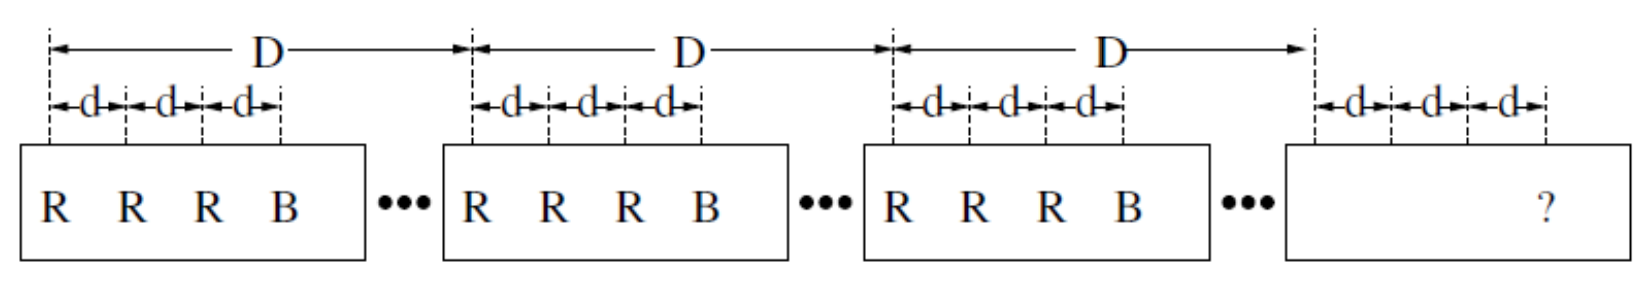
\includegraphics[width=0.7\textwidth]{par50vdw44.png}
    \end{center}

    Если $\chi(a + 3D + 3d) = B$, то 
    
    \[ \chi(a + 3d) = \chi(a + D + 3d) = \chi(a + 2D + 3d) = \chi(a + 3D + 3d) = B. \]

    Если $\chi(a + 3D + 3d) = R$, то

    \[ \chi(a + 3d) = \chi(a) = \chi(a + D + d) = \chi(a + 2D + 2d) = \chi(a + 3D + 3d) = R. \]

    В любом случае получили одноцветную $4$-а.п.

\end{proof}

\end{normalsize}
